
%-----------------------------------------------------------------------------------------------------------------------------------------------%
%	The MIT License (MIT)
%
%	Copyright (c) 2019 Jan Küster
%
%	Permission is hereby granted, free of charge, to any person obtaining a copy
%	of this software and associated documentation files (the "Software"), to deal
%	in the Software without restriction, including without limitation the rights
%	to use, copy, modify, merge, publish, distribute, sublicense, and/or sell
%	copies of the Software, and to permit persons to whom the Software is
%	furnished to do so, subject to the following conditions:
%	
%	THE SOFTWARE IS PROVIDED "AS IS", WITHOUT WARRANTY OF ANY KIND, EXPRESS OR
%	IMPLIED, INCLUDING BUT NOT LIMITED TO THE WARRANTIES OF MERCHANTABILITY,
%	FITNESS FOR A PARTICULAR PURPOSE AND NONINFRINGEMENT. IN NO EVENT SHALL THE
%	AUTHORS OR COPYRIGHT HOLDERS BE LIABLE FOR ANY CLAIM, DAMAGES OR OTHER
%	LIABILITY, WHETHER IN AN ACTION OF CONTRACT, TORT OR OTHERWISE, ARISING FROM,
%	OUT OF OR IN CONNECTION WITH THE SOFTWARE OR THE USE OR OTHER DEALINGS IN
%	THE SOFTWARE.
%	
%
%-----------------------------------------------------------------------------------------------------------------------------------------------%


%============================================================================%
%
%	DOCUMENT DEFINITION
%
%============================================================================%

\documentclass[10pt,A4,english]{article}	


%----------------------------------------------------------------------------------------
%	ENCODING
%----------------------------------------------------------------------------------------

% we use utf8 since we want to build from any machine
\usepackage[utf8]{inputenc}		
\usepackage[USenglish]{isodate}
\usepackage{fancyhdr}
\usepackage[numbers]{natbib}

%----------------------------------------------------------------------------------------
%	LOGIC
%----------------------------------------------------------------------------------------

% provides \isempty test
\usepackage{xstring, xifthen}
\usepackage{enumitem}
\usepackage[english]{babel}
\usepackage{blindtext}
\usepackage{pdfpages}
\usepackage{changepage}
%----------------------------------------------------------------------------------------
%	FONT BASICS
%----------------------------------------------------------------------------------------

% some tex-live fonts - choose your own

%\usepackage[defaultsans]{droidsans}
%\usepackage[default]{comfortaa}
%\usepackage{cmbright}
\usepackage[default]{raleway}
%\usepackage{fetamont}
%\usepackage[default]{gillius}
%\usepackage[light,math]{iwona}
%\usepackage[thin]{roboto} 

% set font default
\renewcommand*\familydefault{\sfdefault} 	
\usepackage[T1]{fontenc}

% more font size definitions
\usepackage{moresize}

%----------------------------------------------------------------------------------------
%	FONT AWESOME ICONS
%---------------------------------------------------------------------------------------- 

% include the fontawesome icon set
\usepackage{fontawesome}

% use to vertically center content
% credits to: http://tex.stackexchange.com/questions/7219/how-to-vertically-center-two-images-next-to-each-other
\newcommand{\vcenteredinclude}[1]{\begingroup
\setbox0=\hbox{\includegraphics{#1}}%
\parbox{\wd0}{\box0}\endgroup}
\newcommand{\tab}[1]{\hspace{.2\textwidth}\rlap{#1}}
% use to vertically center content
% credits to: http://tex.stackexchange.com/questions/7219/how-to-vertically-center-two-images-next-to-each-other
\newcommand*{\vcenteredhbox}[1]{\begingroup
\setbox0=\hbox{#1}\parbox{\wd0}{\box0}\endgroup}

% icon shortcut
\newcommand{\icon}[3] { 							
	\makebox(#2, #2){\textcolor{maincol}{\csname fa#1\endcsname}}
}	


% icon with text shortcut
\newcommand{\icontext}[4]{ 						
	\vcenteredhbox{\icon{#1}{#2}{#3}}  \hspace{2pt}  \parbox{0.9\mpwidth}{\textcolor{#4}{#3}}
}

% icon with website url
\newcommand{\iconhref}[5]{ 						
    \vcenteredhbox{\icon{#1}{#2}{#5}}  \hspace{2pt} \href{#4}{\textcolor{#5}{#3}}
}

% icon with email link
\newcommand{\iconemail}[5]{ 						
    \vcenteredhbox{\icon{#1}{#2}{#5}}  \hspace{2pt} \href{mailto:#4}{\textcolor{#5}{#3}}
}

%----------------------------------------------------------------------------------------
%	PAGE LAYOUT  DEFINITIONS
%----------------------------------------------------------------------------------------

% page outer frames (debug-only)
% \usepackage{showframe}		

% we use paracol to display breakable two columns
\usepackage{paracol}
\usepackage{tikzpagenodes}
\usetikzlibrary{calc}
\usepackage{lmodern}
\usepackage{multicol}
\usepackage{lipsum}
\usepackage{atbegshi}
% define page styles using geometry
\usepackage[a4paper]{geometry}

% remove all possible margins
\geometry{top=1cm, bottom=1cm, left=1cm, right=1cm}

\usepackage{fancyhdr}
\pagestyle{empty}

% space between header and content
% \setlength{\headheight}{0pt}

% indentation is zero
\setlength{\parindent}{0mm}

%----------------------------------------------------------------------------------------
%	TABLE /ARRAY DEFINITIONS
%---------------------------------------------------------------------------------------- 

% extended aligning of tabular cells
\usepackage{array}

% custom column right-align with fixed width
% use like p{size} but via x{size}
\newcolumntype{x}[1]{%
>{\raggedleft\hspace{0pt}}p{#1}}%


%----------------------------------------------------------------------------------------
%	GRAPHICS DEFINITIONS
%---------------------------------------------------------------------------------------- 

%for header image
\usepackage{graphicx}

% use this for floating figures
% \usepackage{wrapfig}
% \usepackage{float}
% \floatstyle{boxed} 
% \restylefloat{figure}

%for drawing graphics		
\usepackage{tikz}			
\usepackage{ragged2e}	
\usetikzlibrary{shapes, backgrounds,mindmap, trees}

%----------------------------------------------------------------------------------------
%	Color DEFINITIONS
%---------------------------------------------------------------------------------------- 
\usepackage{transparent}
\usepackage{color}

% primary color
\definecolor{maincol}{RGB}{ 64,64,64}

% accent color, secondary
% \definecolor{accentcol}{RGB}{ 250, 150, 10 }

% dark color
\definecolor{darkcol}{RGB}{ 70, 70, 70 }

% light color
\definecolor{lightcol}{RGB}{245,245,245}

\definecolor{accentcol}{RGB}{59,77,97}



% Package for links, must be the last package used
\usepackage[hidelinks]{hyperref}

% returns minipage width minus two times \fboxsep
% to keep padding included in width calculations
% can also be used for other boxes / environments
\newcommand{\mpwidth}{\linewidth-\fboxsep-\fboxsep}
	


%============================================================================%
%
%	CV COMMANDS
%
%============================================================================%

%----------------------------------------------------------------------------------------
%	 CV LIST
%----------------------------------------------------------------------------------------

% renders a standard latex list but abstracts away the environment definition (begin/end)
\newcommand{\cvlist}[1] {
	\begin{itemize}{#1}\end{itemize}
}

%----------------------------------------------------------------------------------------
%	 CV TEXT
%----------------------------------------------------------------------------------------

% base class to wrap any text based stuff here. Renders like a paragraph.
% Allows complex commands to be passed, too.
% param 1: *any
\newcommand{\cvtext}[1] {
	\begin{tabular*}{1\mpwidth}{p{0.98\mpwidth}}
		\parbox{1\mpwidth}{#1}
	\end{tabular*}
}
\newcommand{\cvtextsmall}[1] {
	\begin{tabular*}{0.8\mpwidth}{p{0.8\mpwidth}}
		\parbox{0.8\mpwidth}{#1}
	\end{tabular*}
}
%----------------------------------------------------------------------------------------
%	CV SECTION
%----------------------------------------------------------------------------------------

% Renders a a CV section headline with a nice underline in main color.
% param 1: section title
\newlength{\barw}
\newcommand{\cvsection}[1] {
	\vspace{14pt}
	\settowidth{\barw}{\textbf{\LARGE #1}}
	\cvtext{
		\textbf{\LARGE{\textcolor{darkcol}{#1}}}\\[-4pt]
		\textcolor{accentcol}{ \rule{\barw}{1.5pt} } \\
	}
}

\newcommand{\cvsubsection}[1] {
	\vspace{14pt}
	\settowidth{\barw}{\textbf{\Large #1}}
	\cvtext{
		\textbf{\Large{\textcolor{darkcol}{#1}}}\\[-4pt]
		\textcolor{accentcol}{ \rule{\barw}{1.5pt} } \\
	}
}

\newcommand{\cvheadline}[1] {
	\vspace{16pt}
	\cvtext{
		\textbf{\Huge{\textcolor{accentcol}{#1}}}\\[-4pt]
		 
	}
}

\newcommand{\cvsubheadline}[1] {
	\vspace{16pt}
	\cvtext{
		\textbf{\huge{\textcolor{darkcol}{#1}}}\\[-4pt]
		 
	}
}
%----------------------------------------------------------------------------------------
%	META SKILL
%----------------------------------------------------------------------------------------

% Renders a progress-bar to indicate a certain skill in percent.
% param 1: name of the skill / tech / etc.
% param 2: level (for example in years)
% param 3: percent, values range from 0 to 1
\newcommand{\cvskill}[3] {
	\begin{tabular*}{1\mpwidth}{p{0.72\mpwidth}  r}
 		\textcolor{black}{\textbf{#1}} & \textcolor{maincol}{#2}\\
	\end{tabular*}%
	
	\hspace{4pt}
	\begin{tikzpicture}[scale=1,rounded corners=2pt,very thin]
		\fill [lightcol] (0,0) rectangle (1\mpwidth, 0.15);
		\fill [accentcol] (0,0) rectangle (#3\mpwidth, 0.15);
  	\end{tikzpicture}%
}


%----------------------------------------------------------------------------------------
%	 CV EVENT
%----------------------------------------------------------------------------------------

% Renders a table and a paragraph (cvtext) wrapped in a parbox (to ensure minimum content
% is glued together when a pagebreak appears).
% Additional Information can be passed in text or list form (or other environments).
% the work you did
% param 1: time-frame i.e. Sep 14 - Jan 15 etc.
% param 2:	 event name (job position etc.)
% param 3: Customer, Employer, Industry
% param 4: Short description
% param 5: work done (optional)
% param 6: technologies include (optional)
% param 7: achievements (optional)
\newcommand{\cvevent}[7] {
	
	% we wrap this part in a parbox, so title and description are not separated on a pagebreak
	% if you need more control on page breaks, remove the parbox
	\parbox{\mpwidth}{
		\begin{tabular*}{1\mpwidth}{p{0.66\mpwidth}  r}
	 		\textcolor{black}{\textbf{#2}} & \colorbox{accentcol}{\makebox[0.32\mpwidth]{\textcolor{white}{\textbf{#1}}}} \\
			\textcolor{maincol}{#3} & \\
		\end{tabular*}\\[8pt]
	
		\ifthenelse{\isempty{#4}}{}{
			\cvtext{#4}\\
		}
	}
	\vspace{14pt}
}


%----------------------------------------------------------------------------------------
%	 CV META EVENT
%----------------------------------------------------------------------------------------

% Renders a CV event on the sidebar
% param 1: title
% param 2: subtitle (optional)
% param 3: customer, employer, etc,. (optional)
% param 4: info text (optional)
\newcommand{\cvmetaevent}[4] {
	\textcolor{maincol} { \cvtext{\textbf{\begin{flushleft}#1\end{flushleft}}}}

	\ifthenelse{\isempty{#2}}{}{
	\textcolor{black} {\cvtext{\textbf{#2}} }
	}

	\ifthenelse{\isempty{#3}}{}{
		\cvtext{{ \textcolor{maincol} {#3} }}\\
	}

	\cvtext{#4}\\[14pt]
}

%---------------------------------------------------------------------------------------
%	QR CODE
%----------------------------------------------------------------------------------------

% Renders a qrcode image (centered, relative to the parentwidth)
% param 1: percent width, from 0 to 1
\newcommand{\cvqrcode}[1] {
	\begin{center}
		\includegraphics[width={#1}\mpwidth]{qrcode}
	\end{center}
}


% HEADER AND FOOOTER 
%====================================
\newcommand\Header[1]{%
\begin{tikzpicture}[remember picture,overlay]
\fill[accentcol]
  (current page.north west) -- (current page.north east) --
  ([yshift=50pt]current page.north east|-current page text area.north east) --
  ([yshift=50pt,xshift=-3cm]current page.north|-current page text area.north) --
  ([yshift=10pt,xshift=-5cm]current page.north|-current page text area.north) --
  ([yshift=10pt]current page.north west|-current page text area.north west) -- cycle;
\node[font=\sffamily\bfseries\color{white},anchor=west,
  xshift=0.7cm,yshift=-0.32cm] at (current page.north west)
  {\fontsize{12}{12}\selectfont {#1}};
\end{tikzpicture}%
}

\newcommand\Footer[1]{%
\begin{tikzpicture}[remember picture,overlay]
\fill[lightcol]
  (current page.south east) -- (current page.south west) --
  ([yshift=-80pt]current page.south east|-current page text area.south east) --
  ([yshift=-80pt,xshift=-6cm]current page.south|-current page text area.south) --
  ([xshift=-2.5cm,yshift=-10pt]current page.south|-current page text area.south) --	
  ([yshift=-10pt]current page.south east|-current page text area.south east) -- cycle;
\node[yshift=0.32cm,xshift=9cm] at (current page.south) {\fontsize{10}{10}\selectfont \textbf{\thepage}};
\end{tikzpicture}%
}


%=====================================
%============================================================================%
%
%
%
%	DOCUMENT CONTENT
%
%
%
%============================================================================%
\begin{document}

\columnratio{0.31}
\setlength{\columnsep}{2.2em}
\setlength{\columnseprule}{4pt}
\colseprulecolor{white}


% LEBENSLAUF HIERE
\AtBeginShipoutFirst{\Header{CV}\Footer{1}}
\AtBeginShipout{\AtBeginShipoutAddToBox{\Header{CV}\Footer{2}}}

\newpage

\colseprulecolor{lightcol}
\columnratio{0.31}
\setlength{\columnsep}{2.2em}
\setlength{\columnseprule}{4pt}
\begin{paracol}{2}


\begin{leftcolumn}
%---------------------------------------------------------------------------------------
%	META IMAGE
%----------------------------------------------------------------------------------------
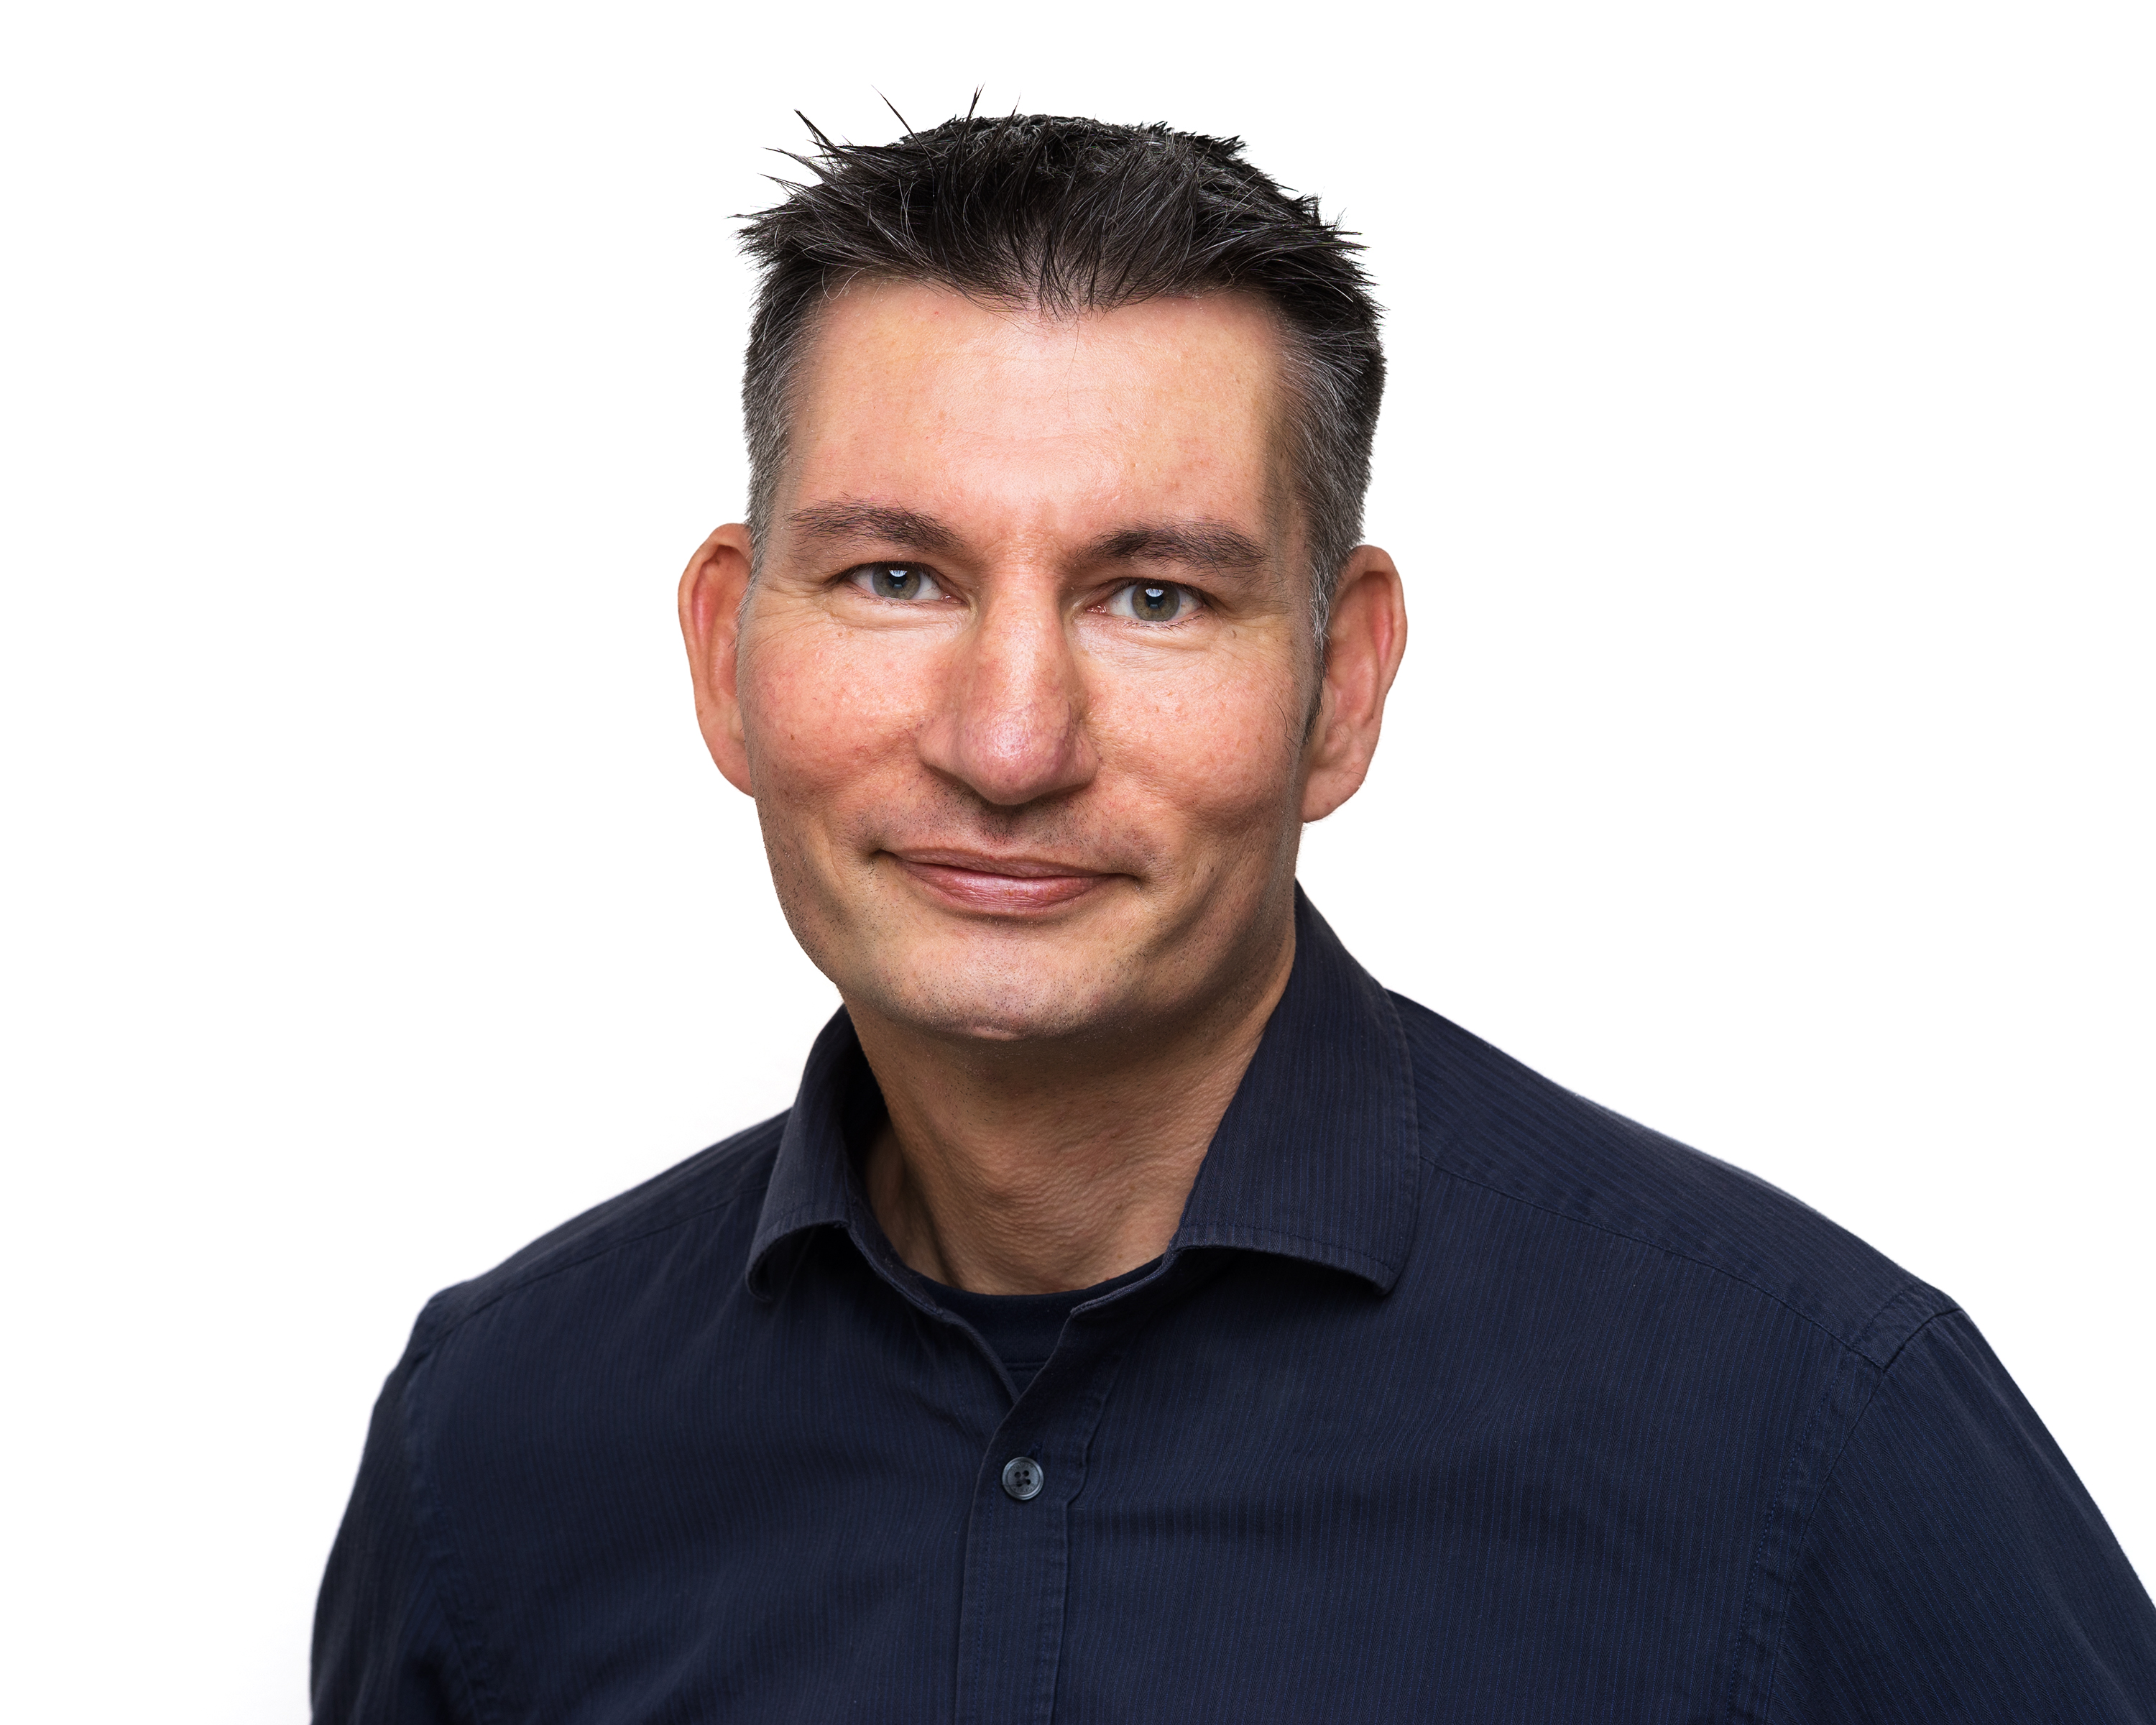
\includegraphics[width=\linewidth]{resources/me.jpg}	%trimming relative to image size

%---------------------------------------------------------------------------------------
%	META SKILLS
%----------------------------------------------------------------------------------------
	\fcolorbox{white}{white}{\begin{minipage}[c][1.5cm][c]{1\mpwidth}
		\LARGE{\textbf{\textcolor{maincol}{Mikael Vatau}}} \\[2pt]
		\normalsize{ \textcolor{maincol} {Software Developer} }
\end{minipage}} \\
\icontext{CaretRight}{12}{Swedish}{black}\\[6pt]
\icontext{CaretRight}{12}{Unmarried}{black}\\[6pt]



\cvsection{Skills}

\cvskill{Software development} {13l+ Years} {1} \\[-2pt]

\cvskill{Customer service} {7+ Years} {1} \\[-2pt]

\cvskill{Embedded systems} {8+ yrs.} {0.8} \\[-2pt]

\cvskill{Linux} {15+ yrs.} {0.8} \\[-2pt]

\cvskill{Web development} {2+ yrs.} {0.32} \\[-2pt]

\cvskill{C / C++} {10+ yrs.} {0.9} \\[-2pt]

\cvskill{PHP} {2+ yrs.} {0.4} \\[-2pt]

\cvskill{Python} {2+ yrs.} {0.4} \\[-2pt] \\

\cvskill{Swedish} {L1} {1} \\[-2pt]

\cvskill{English} {C1} {0.9} \\[-2pt]


\newpage
%---------------------------------------------------------------------------------------
%	EDUCATION
%----------------------------------------------------------------------------------------

\cvsection{Interests}

\icontext{CaretRight}{12}{Piano}{black}\\[6pt]
\icontext{CaretRight}{12}{Chess}{black}\\[6pt]
\icontext{CaretRight}{12}{Travel}{black}\\[6pt]




\cvsection{Contact}

\icontext{MapMarker}{16}{Rua Heliodoro 22a\\1170-177 Lisbon}{black}\\[6pt]
\icontext{MobilePhone}{16}{+351 926 888 037}{black}\\[6pt]
\iconemail{Envelope}{16}{sleepbrunch@gmail.com}{XXXX@XXXXX.XX}{black}\\[6pt]
\iconhref{Github}{16}{github.com/secratry}{https://www.github.com/secratry}{black}\\[6pt]
%\iconhref{Xing}{16}{xing.com/user\_name}{https://www.xing.com/profile/User_Name}{black}\\

	
%\cvqrcode{0.3}

\end{leftcolumn}
\begin{rightcolumn}
%---------------------------------------------------------------------------------------
%	TITLE  HEADER
%----------------------------------------------------------------------------------------


%---------------------------------------------------------------------------------------
%	PROFILE
%----------------------------------------------------------------------------------------
\cvsection{Biography}
\vspace{4pt}

\cvtext{Eight years experience developing mobile phone platform and
almost 13 year experience in embedded system development both hardware and software. Worked with audio, GPS, touchscreen, Bluetooth,
WLAN and motor control in large and small scaled project. Seven years
experience in customer care.
}


%---------------------------------------------------------------------------------------
%	WORK EXPERIENCE
%----------------------------------------------------------------------------------------

\vspace{10pt}
\cvsection{Work experience}
\vspace{4pt}


\cvevent
{Sep 2017 - Oct 2023}
	{Technical Support} 
	{Accenture}
	{Technical support for Google Adwords and Analytics}
	\vfill\null

\cvevent
{Aug 2016 - Oct 2017}
	{Customer Support}
	{CGI Portugal}
	{Supporting both interal and customer in IT}
	\vfill\null

\cvevent
	{Sep 2015 - Aug 2019}
	{Customer Support} 
	{Teleperformance}
	{Supporting Swedish customers (Photobox, Boxer)}
	\vfill\null

\cvevent
	{Mar 2005 - Apr 2019}
	{Software Consultant}
	{Netville AB}
	{I was involved in software configuration, low-level audio development, GPS, touch screen, WLAN, Bluetooth, on-site technical support, and application development during my 8-year tenure at Netville:
	\begin{itemize}
		\item Camera Web Interface Development (5 months) at Axis Communications for their security cameras.
		\item Platform-Based Applications Development (1 year) at Sony Ericsson: Collaborated on Android applications, such as the calendar, and clock in a small team of 2 that expanded to eight members and 10 applications.
		\item Low-Level Audio Development (2 years) at ST-Ericsson: Involved development for Low Power audio, Wideband Bluetooth, and ALSA, including providing on-site support in Asia and Sweden.
		\item Accessibility App Development (3 months) for Netville Customer: Developed an Android application aiding visually impaired individuals.
		\item Test Software Development (1 year) at Sony Ericsson Mobile Communications AB: to be run on phone to test the GPS signal-to-noise redusing the test time from 30 to 4 seconds.
		\item Configuration Management and Development (4 years) at Ericsson AB: Initially serving as Configuration Manager, later transitioning into a developer role within the Open Platform Architecture department in addition to configuringand supporting PC-lint tool.
	\end{itemize} }
	\vfill\null

\cvevent
	{Jan 2000 - Sep 2004}
	{Research Engineer}
	{Robotics Lunds, University}
	{Worked almost 5 years in multiple hardware and software projects, Maintaining of the departments computer and with development of their website.
	\begin{itemize}
		\item Network administration of the departments computers. (IRIX, Linux, and Windows)
		\item Assisted in developing the departments new website (news page and document repository).
		\item Assisted in developing the departments new website (news page and document repository).
		\item Implement, verify and troubleshot controller cards based on 32bit Freescale CPU for DC and Step motor control.
		\item Implement, verify and troubleshot controller cards based on 32bit Freescale CPU for DC and Step motor control.
		\item Hardware and software for controllers to be used in on a robotics arm on attached to a wheelchair (they used the CAN protocoll for communication). 
		\item Worked with an EU project, designing and implementing the controllers and software to be used in bottle openers for physically disabled people. 
	\end{itemize}}
	\vfill\null



\cvsection{Education}
\begin{itemize}[leftmargin=*]

\item 2009, SEMC AB (EMEA) Linux for Embedded Systems Advanced

\item 2008, Ericsson AB Linux for Embedded Systems

\item 2006, Ericsson AB GPRS Security

\item 2003, Malmo University Practical English in Cross-cultural Communications

\item 2000, SGI IRIX System Administration

\item 1997 - 2000, Lunds Institute of Technology B.Sc.E. Electro Engineer
\end{itemize}




\cvsection{Publications}

\begin{itemize}[leftmargin=*]
\item Author, G. \& Author, P. \&  Author G. (2020). "This is the title of the publication". In: \textit{Proceedings of the 28th Conference on Lipsum (LIPSUM)}, Lipsum, June 12-17, 2020.
\item Author, G. \& Author, P. \&  Author G. (2020). "This is the title of the publication". In: \textit{Proceedings of the 28th Conference on Lipsum (LIPSUM)}, Lipsum, June 12-17, 2020.
\item Author, G. \& Author, P. \&  Author G. (2020). "This is the title of the publication". In: \textit{Proceedings of the 28th Conference on Lipsum (LIPSUM)}, Lipsum, June 12-17, 2020.
\end{itemize}
% hofixes to create fake-space to ensure the whole height is used
\mbox{}
\vfill
\mbox{}
\vfill
\mbox{}
\vfill
\mbox{}
\vfill
\mbox{}
\vfill
\mbox{}
\vfill
\mbox{}


\end{rightcolumn}
\end{paracol}


\end{document}
